\section{Replica Symmetry Breaking, Neural Nets, Boltzmann Machines}

\emph{I was absent for this lecture, and these lecture notes are obtained from Kalpak Duddella's notes - many thanks to him!}

In this lecture, we wrap up the discussion of spin glasses and replica symmetry breaking, before moving onto the last topic of discussion for this course - Neural networks and Boltzmann machines.

\subsection{Replica Symmetry Breaking, Concluded}
We consider the replica matrix ansatz $Q_{ab}$, as you will study in HW3. Its structure ``naturally clusters'' due to off-diagonal (correlation) elements, forming a block structure about the diagonal. We obtain this by guessing the block form as the solution to the non-linear EoM and minimizing the free energy. But, we also have to check the stability of the solutions.

In more detail, we have 1s on the diagonal, $q_1$ in $m \times m$ blocks around the diagonal, and $q_0$ elsewhere, with $1 > q_1 > q_0$. We have the probability distribution:
\begin{equation}
    P(q) = \frac{m-1}{n-1}\delta(q - q_1) + \frac{n-m}{n-1}\delta(q - q_0)
\end{equation}
which as $n \to 0$ becomes the two delta peaks:
\begin{equation}
    p(q) = (1-m)\delta(q - q_1) + m\delta(q - q_0)
\end{equation}
Graphically, we have the distribution as sketched last class. In this limit, we have 1-step symmetry breaking in the exact solution of the $p$-spin spherical model.

\begin{center}
    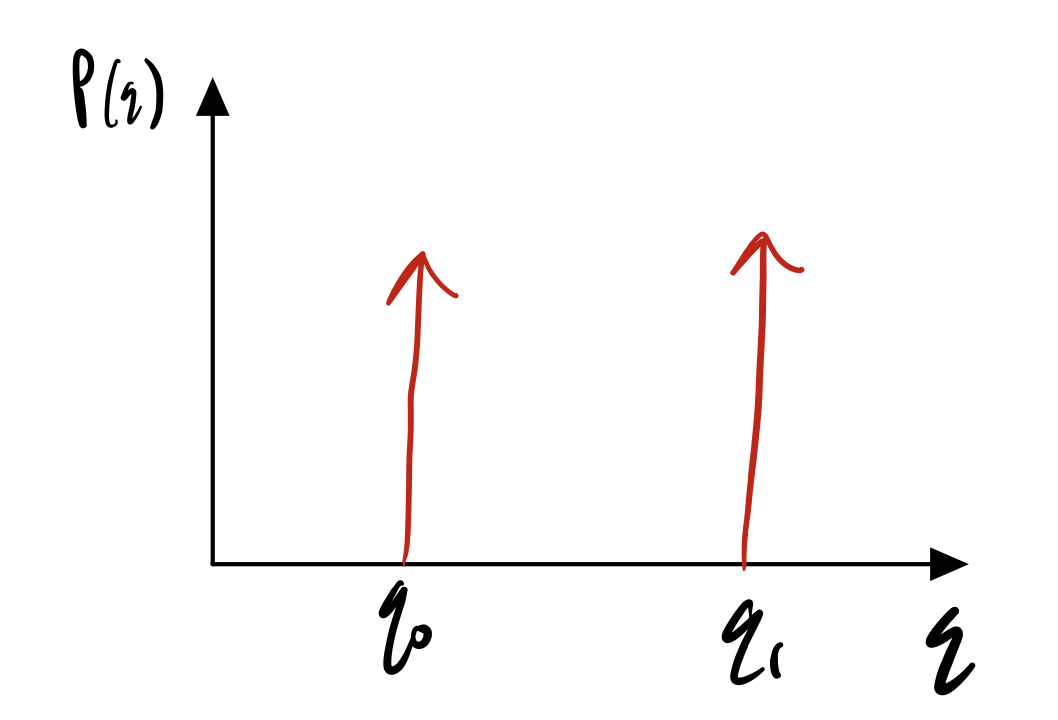
\includegraphics[scale=0.35]{Lectures/Figures/lec15-1stepsymbreak.png}
\end{center}

For $T < T_s$, we have a continuous solution where $P(a)$ varies smoothly between the two peaks at $q_0, q_1$, with peaks getting closer together as $T \to T_s$.

\begin{center}
    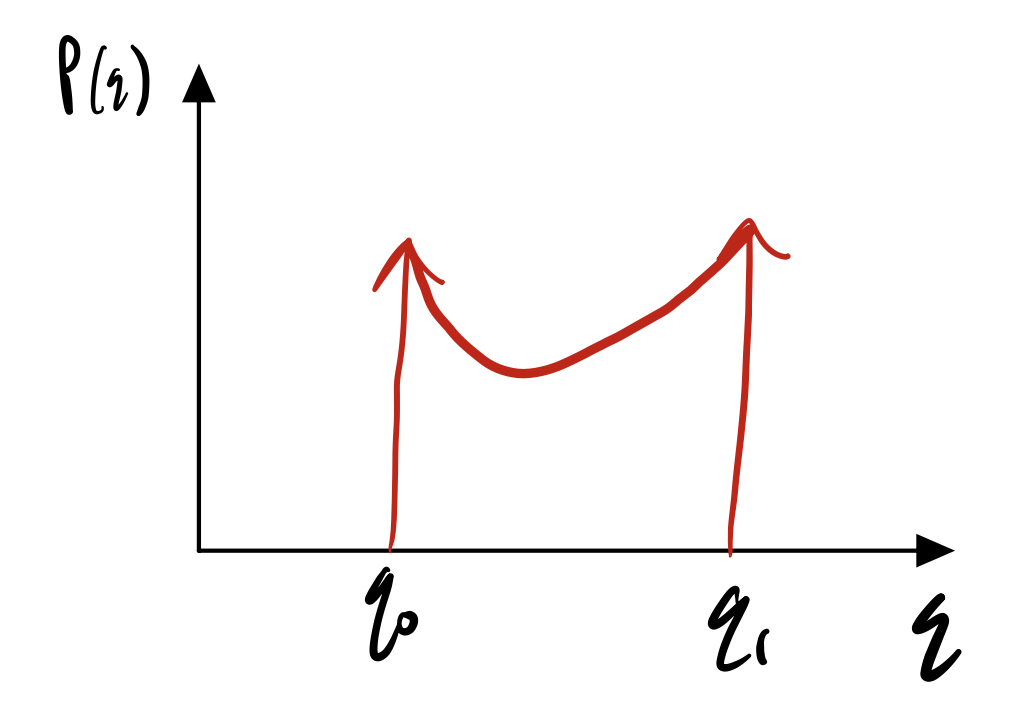
\includegraphics[scale=0.35]{Lectures/Figures/lec15-TleqTs.png}
\end{center}

For $T > T_c$, we have ``ultrametricity''; full replica symmetry breaking.

\begin{center}
    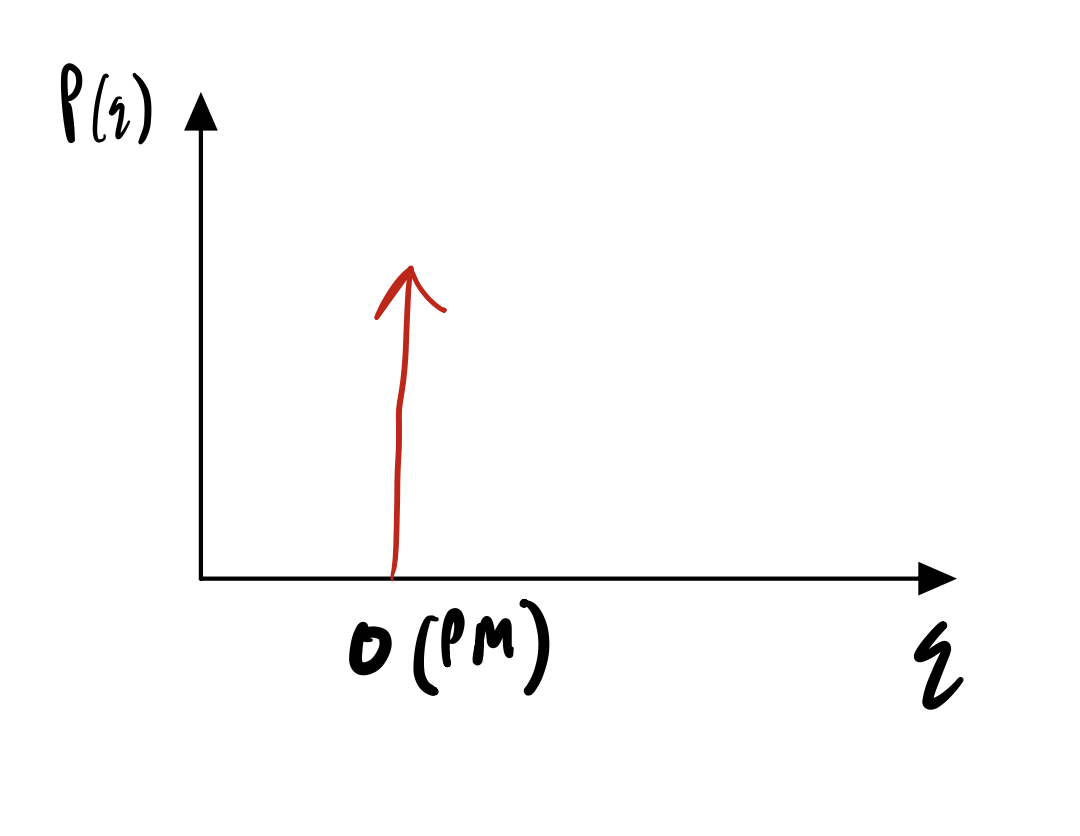
\includegraphics[scale=0.35]{Lectures/Figures/lec15-TgeqTs.png}
\end{center}

This is related to lines connecting points on the $\dpd{F}{Q}$ curve.

\begin{center}
    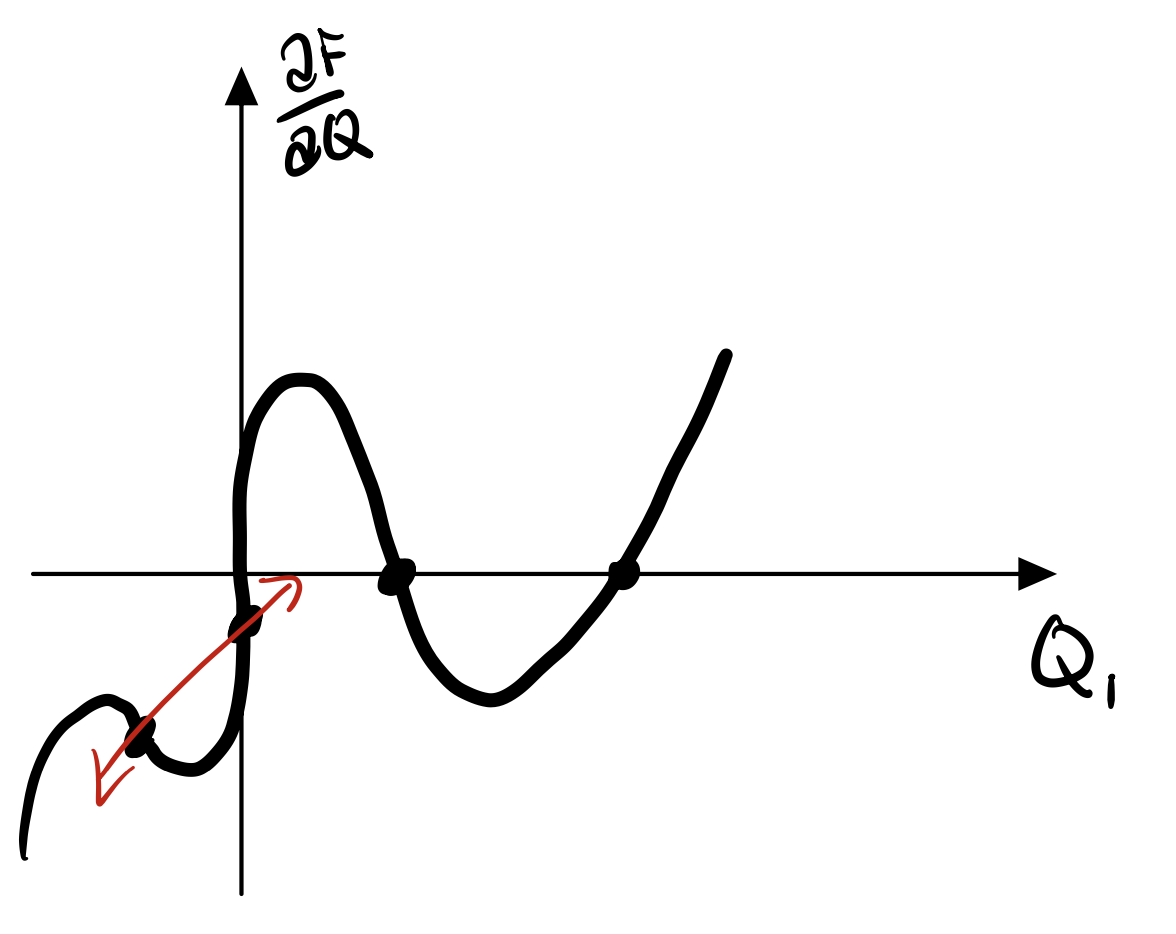
\includegraphics[scale=0.35]{Lectures/Figures/lec15-dFdQ.png}
\end{center}

\subsection{Neural Nets}
John Hopfield considered the following model for associative memory - consider the vector $\gv{\chi}$. We then store this memory by flipping spins in an (Ising) array, with system Hamiltonian:
\begin{equation}
    H = -\sum_{\avg{ij}}J_{ij}S_iS_j
\end{equation}
where the couplings are:
\begin{equation}
    J_{ij} = J\xi_i\xi_j
\end{equation}
Thus:
\begin{equation}
    H = -J\sum_i \xi_i S_i \sum_j \xi_j S_j
\end{equation}
If we now generalize to store a set of bit strings $\set{\chi^a}_a$. Then for an associative memory, we take:
\begin{equation}
    J_{ij} = \sum_a \chi_i^a \chi_j ^a
\end{equation}
with $a$ indexing over different bitstrings and $i$ indexing the position in a given bitstring. This is a ``one-layer neural network'' (we take $1 = \uparrow$, $0 = \downarrow$). Hopfield won a Nobel for a (insert choice word) ferromagnet!

For a $N \times N$ neural network, we can store about $\sim 0.15N$ memories. 

\subsection{Boltzmann Machines}
Two step phases for using Boltzmann machines:
\begin{enumerate}
    \item We first run a training phase to obtain the $\xi_i$.
    \item We then run a readout phase to allow the system to evolve on a fixed array of $J$s constructed from the learned $\xi$s.
\end{enumerate}

We consider the probability weights for a given spin configuration $s$
\begin{equation}
    P(s) = \exp(-E(s))/Z
\end{equation}
where the energy function is:
\begin{equation}
    E(s) = \sum_{ij}U_{ij}s_is_j - \sum_i b_i s_i
\end{equation}
with $U_{ij}$ the weights and $b_i$ the biases. We need to \emph{learn} the $U$s and $b$s to have the model $P(s)$ fit the data, i.e.:
\begin{equation}
    \left.P(s)\right|_{\text{model}} \approx \left.P(s)\right|_{\text{data}}.
\end{equation}

Comparing neural networks with spin models, a layered neural network corresponds to an auxiliary field model.

\begin{center}
    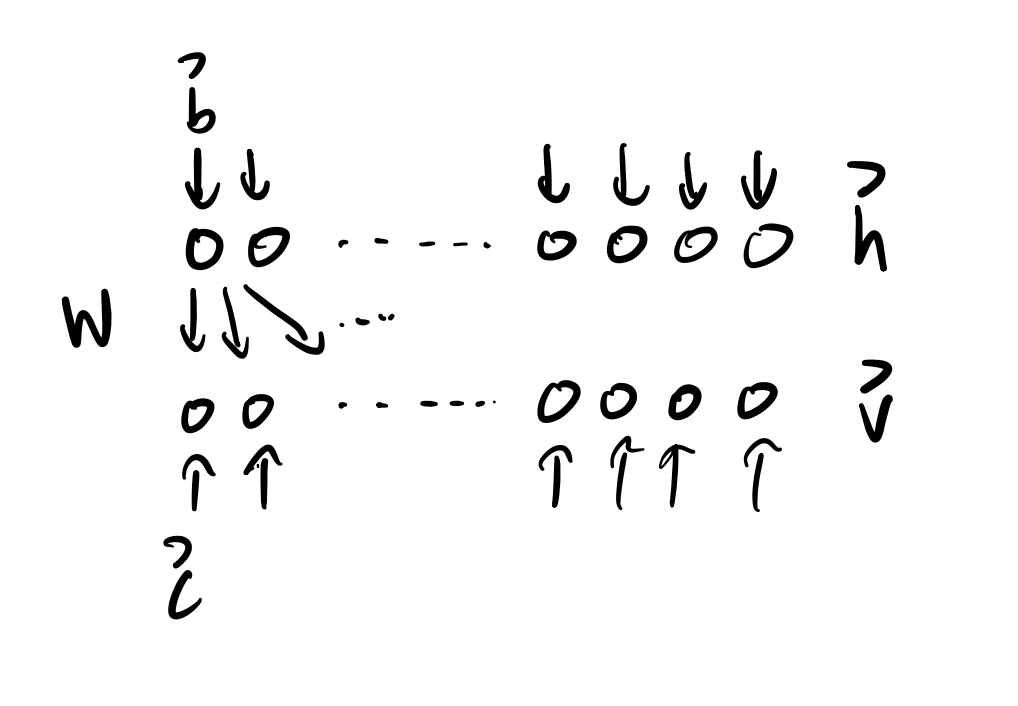
\includegraphics[scale=0.35]{Lectures/Figures/lec15-NN.png}
\end{center}

For simplicity, we consider a 2-layer network, composed of a hidden layer of nodes (vector of spins) $\v{h}$ and a visible layers of nodes $\v{v}$. We have a bias $\v{b}$ on the hidden nodes and $\v{c}$ on the visible nodes. We also have a weight-matrix $W$ between the two layers which computes ``scores'' as a linear transformation.

The energy of a neuron configuration specified by $\v{v}, \v{h}$ is:
\begin{equation}
    E(v, h) = -\v{b} \cdot \v{v} - \v{c} \cdot \v{h} - v_iW_{ij}jh_j
\end{equation}
We then have the conditional probabilities:
\begin{equation}
    P(\v{h} \vert \v{v}) = \prod_i P(h_i \vert \v{v})
\end{equation}
\begin{equation}
    P(\v{v} \vert \v{h}) = \prod_i P(v_i \vert \v{h})
\end{equation}
Which we can also write as:
\begin{equation}
    P(\v{h} \vert \v{v}) = \frac{P(\v{h}, \v{v})}{P(\v{v})} = \frac{1}{P(\v{v})Z}e^{\v{b} \cdot \v{v} + \v{c} \cdot \v{h} + v_iW_{ij}h_j} = \frac{1}{Z'}e^{\v{c} \cdot \v{h} + v_iW_{ij}h_j}
\end{equation}
With $\frac{1}{Z'} = \frac{1}{P(v)Z}e^{\v{b} \cdot \v{v}}$. 

Now, we have some data probability ditribution $P_{\text{data}}(\v{x})$. We have a model probability distribution $P_{\text{model}}(\v{x};\gv{\theta})$ with model parameters $\gv{\theta}$. The goal is to find the optimal model parameters, obtained from:
\begin{equation}
    \gv{\theta}_{\text{model}} = \text{argmax}_{\theta}\prod_{i=1}^m P_{\text{model}}(x_i, \theta) = \sum_{i=1}^m \log P_{\text{model}}(x_i, \theta)
\end{equation}